\subsubsection{14.01.2016}
\textit{\textbf{Time frame:}} 19:00-21:00

There were found two reasons of the problem of the elevator.

Firstly, the battery at the previous test was low. 

Secondly, the ribs that connect two sides of the elevator caused a bend. it was because the cables at both sides were not the same length, so the sides of elevator were extracting differently.

To solve this problem, it was decided to make the mounts of the ribs mobile. So if there appear some bend, the ribs will merely slide along the movable mount (a kind of small slat).

%\begin{figure}[H]
%	\begin{minipage}[h]{1\linewidth}
%		\center{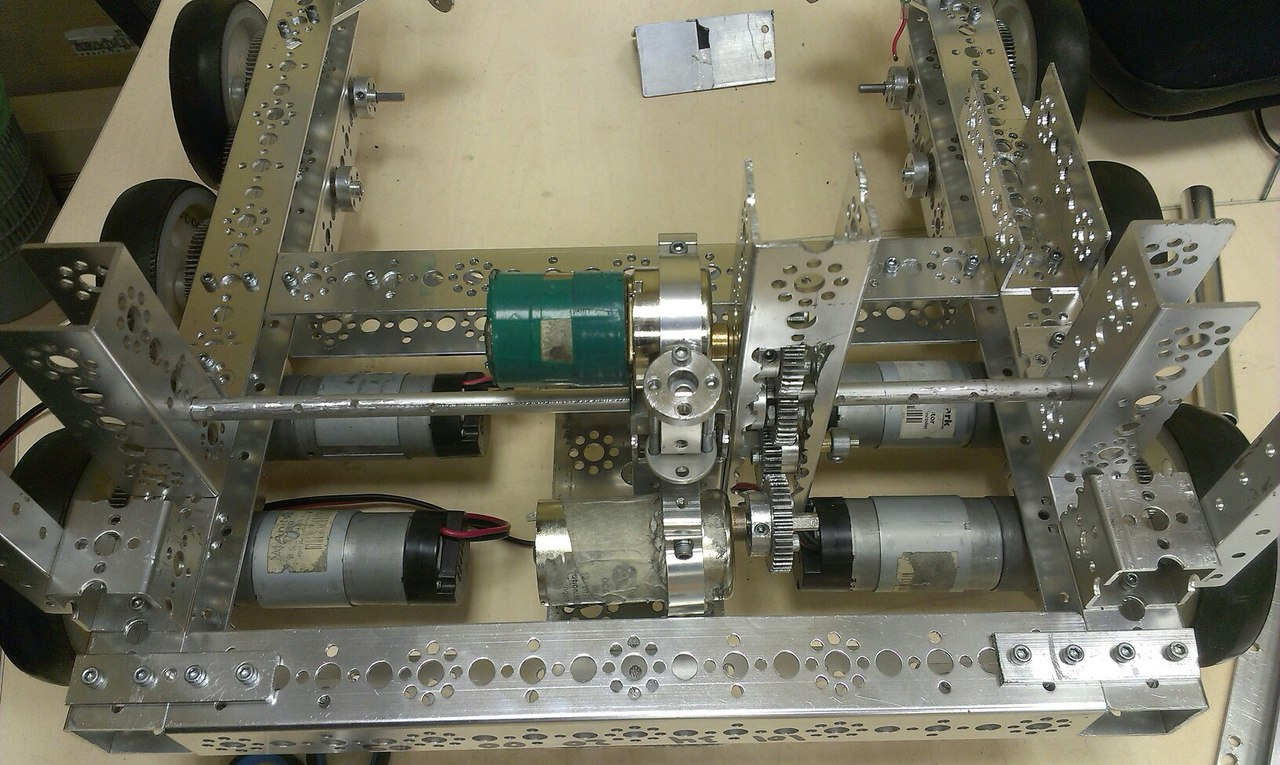
\includegraphics[scale=0.3]{3Engineering/5Team_meetings/days_of_meetings/2016.01.14/images/01}}
%		\caption{}

%	\end{minipage}
%\end{figure}